% !TeX program = xelatex
\documentclass[a4paper,10pt]{article}

% ============================================================================
% សន្លឹកកិច្ចការសិស្សបំពេញចន្លោះ ស-ខ្មៅ និងប្លង់ក្ដារខៀន/ចម្លើយគ្រូ (គ្មាន LCD / គ្មានកន្ត្រៃ)
% មេរៀនទី៥ (២.៤--២.៥)៖ វិធីគុណពហុធា និងវិធីចែកពហុធា — ត្រូវគ្នានឹង LS_Plan_ALG54.tex
% ============================================================================
\usepackage[a4paper, left=1.0cm, right=1.0cm, top=0.75cm, bottom=1.00cm, footskip=0.52cm]{geometry}
\usepackage{amsmath}
\usepackage{unicode-math}
\usepackage{fontspec}
\usepackage{array, colortbl}
\usepackage[table]{xcolor}
\usepackage{enumitem}
\usepackage{pifont}
\usepackage{fancyhdr}
\usepackage{lastpage}
\usepackage{tikz}
\usepackage[most]{tcolorbox}
\usetikzlibrary{calc, arrows.meta, decorations.pathreplacing, positioning, babel}

\makeatletter
\let\@expl@@@mark@update@singlecol@structures@@\relax
\makeatother

\providecommand{\NGSFindFonts}{%
  \IfFileExists{C:/Windows/Fonts/cambria.ttc}{%
    \def\NGSSysPath{C:/Windows/Fonts/}%
    \def\NGSUserPath{C:/Users/KIT/AppData/Local/Microsoft/Windows/Fonts/}%
  }{%
    \IfFileExists{./fonts/KhmerOSsiemreap.ttf}{\def\NGSSysPath{./fonts/}\def\NGSUserPath{./fonts/}}{%
    \IfFileExists{../fonts/KhmerOSsiemreap.ttf}{\def\NGSSysPath{../fonts/}\def\NGSUserPath{../fonts/}}{%
    \IfFileExists{../../fonts/KhmerOSsiemreap.ttf}{\def\NGSSysPath{../../fonts/}\def\NGSUserPath{../../fonts/}}{%
    \IfFileExists{../../../fonts/KhmerOSsiemreap.ttf}{\def\NGSSysPath{../../../fonts/}\def\NGSUserPath{../../../fonts/}}{%
    \IfFileExists{../../../../fonts/KhmerOSsiemreap.ttf}{\def\NGSSysPath{../../../../fonts/}\def\NGSUserPath{../../../../fonts/}}{%
    \IfFileExists{../../../../../fonts/KhmerOSsiemreap.ttf}{\def\NGSSysPath{../../../../../fonts/}\def\NGSUserPath{../../../../../fonts/}}{%
    \IfFileExists{../../../../../../fonts/KhmerOSsiemreap.ttf}{\def\NGSSysPath{../../../../../../fonts/}\def\NGSUserPath{../../../../../../fonts/}}{%
      \def\NGSSysPath{../../../../../../../fonts/}\def\NGSUserPath{../../../../../../../fonts/}%
    }}}}}}}%
  }%
}
\NGSFindFonts

\setmathfont[Path={\NGSSysPath}, FontIndex=1, Scale=1.02]{cambria.ttc}
\defaultfontfeatures{Ligatures=TeX}

\setmainfont[
  Path={\NGSUserPath}, Extension=.ttf, Script=Khmer,
  BoldFont={KhmerOSsiemreap}, BoldFeatures={FakeBold=1.8},
  ItalicFont={KhmerOSsiemreap}, ItalicFeatures={FakeSlant=0.25},
  BoldItalicFont={KhmerOSsiemreap}, BoldItalicFeatures={FakeBold=1.8, FakeSlant=0.25}
]{KhmerOSsiemreap}

\newfontfamily\muol[Path={\NGSUserPath}, Extension=.ttf, Script=Khmer]{KhmerOSmuollight}
\newfontfamily\TimesEn[Path={\NGSSysPath}, Extension=.ttf, BoldFont={timesbd}, ItalicFont={timesi}, BoldItalicFont={timesbi}]{times}
\newfontfamily\CalibriFont[Path={\NGSSysPath}, Extension=.ttf]{calibri}

\XeTeXlinebreaklocale "km"
\XeTeXlinebreakskip = 0pt plus 1pt minus 0.1pt

\definecolor{panelgray}{gray}{0.94}
\definecolor{headgray}{gray}{0.85}

\pagestyle{fancy}
\fancyhf{}
\renewcommand{\headrulewidth}{0pt}
\fancyfoot[L]{\fontsize{7.4pt}{9.5pt}\selectfont អនុវិទ្យាល័យព្រះក្រសាំង \en{|} គ្រូ៖ ហុក ប៊ុនថែន \en{|} មេរៀនទី៥ (២.៤--២.៥) វិធីគុណនិងចែកពហុធា \en{|} ថ្ងៃអង្គារ ទី៨ ខែធ្នូ ឆ្នាំ២០២៦}
\fancyfoot[R]{\fontsize{7.8pt}{10pt}\selectfont ទំព័រ \en{\thepage\ / \pageref{LastPage}}}

\setlength{\parindent}{0pt}
\setlength{\parskip}{0pt}
\setlength{\tabcolsep}{4pt}

\newcommand{\en}[1]{{\TimesEn #1}}
\newcommand{\enbf}[1]{{\TimesEn\bfseries #1}}
\newcommand{\unit}[1]{\,\text{\en{#1}}}
\newcommand{\riel}{\,\text{៛}}
\newcommand{\cnum}[1]{\mbox{\fontsize{10pt}{12pt}\selectfont\ding{\numexpr181+#1\relax}}}
\newcommand{\chkbox}{\tikz[baseline=-0.15ex]\draw[black, line width=0.85pt, fill=white] (0,0) rectangle (0.24cm,0.24cm);}
\newcommand{\ansbox}[1][2.0cm]{\,\tikz[baseline=-0.65ex]\draw[black, line width=0.65pt, fill=white] (0,0) rectangle (#1, 0.42cm);\,}
\newcommand{\dotline}[1][2.2cm]{\makebox[#1]{\dotfill}}

\newcommand{\pagebanner}[2]{%
  \begin{tcolorbox}[
    enhanced, sharp corners, colback=headgray, colframe=black,
    boxrule=1.05pt, boxsep=1pt, top=2.5pt, bottom=2.5pt, left=6pt, right=6pt,
    after skip=3.5pt
  ]
    {\muol\fontsize{9.0pt}{13.2pt}\selectfont #1}\hfill{\fontsize{8.0pt}{11.2pt}\selectfont\textbf{#2}}
  \end{tcolorbox}%
}

\newcommand{\secstrip}[2]{%
  \vspace{3pt}%
  \begin{tcolorbox}[
    enhanced, sharp corners, colback=panelgray, colframe=black,
    boxrule=0.8pt, boxsep=0.8pt, top=2pt, bottom=2pt, left=5pt, right=5pt,
    after skip=3pt
  ]
    {\muol\fontsize{8.5pt}{12.2pt}\selectfont #1}\hfill{\fontsize{7.8pt}{10.8pt}\selectfont\textit{#2}}
  \end{tcolorbox}%
}

\newcolumntype{L}[1]{>{\raggedright\arraybackslash}p{#1}}
\newcolumntype{C}[1]{>{\centering\arraybackslash}p{#1}}

\begin{document}
\fontsize{9.5pt}{14.5pt}\selectfont

% ============================================================================
% ទំព័រទី ១៖ សន្លឹកកិច្ចការសិស្ស (ផ្នែកមុខ៖ E1 -> E2 -> E3)
% ============================================================================
\pagebanner{សន្លឹកកិច្ចការសិស្ស \enbf{(}៥\enbf{.}២\enbf{.}៤\enbf{--}៥\enbf{.}២\enbf{.}៥ វិធីគុណនិងចែកពហុធា\enbf{)} \enbf{--} ផ្នែកមុខ}{ថ្នាក់ទី៨ \en{|} សៀវភៅគោល ទំ.៥៩--៦១}

\begin{tcolorbox}[
  enhanced, sharp corners, colback=white, colframe=black,
  boxrule=0.8pt, boxsep=1.5pt, top=3.5pt, bottom=3.5pt, left=5pt, right=5pt,
  after skip=4pt
]
  \fontsize{9.0pt}{13.0pt}\selectfont
  \textbf{ឈ្មោះសិស្ស៖} \dotline[4.3cm] \quad
  \textbf{សមាជិកក្រុម៖} \dotline[4.3cm] \quad
  \textbf{ថ្នាក់ទី៖} ៨\dotline[0.9cm] \quad
  \textbf{ក្រុមទី៖} \dotline[1.0cm]
\end{tcolorbox}

% --- E1 Engage ---
\secstrip{ផ្នែកទី ១ \enbf{(E1 - Engage)} ៖ បេសកកម្មអន្ទាក់សម្រួលតែតួទី១ ពេលចែកពហុធានឹងឯកធា}{រយៈពេល ៣ នាទី (គូស \ding{51} ក្នុង \chkbox)}

\begin{tcolorbox}[
  enhanced, sharp corners, colback=white, colframe=black,
  boxrule=0.8pt, boxsep=2.5pt, top=4pt, bottom=4pt, left=6pt, right=6pt
]
  គេឱ្យផលចែក $(15x^4 - 30x^6) \div (5x^2) = \dfrac{15x^4 - 30x^6}{5x^2}$ (ទំ.៦០) ។ តើសិស្សរូបណាគណនាបានត្រឹមត្រូវ?\\[3pt]
  \chkbox\ \textbf{សិស្ស ក៖} $\dfrac{15x^4 - 30x^6}{5x^2} = 3x^2 - 30x^6$ \qquad\qquad
  \chkbox\ \textbf{សិស្ស ខ៖} $\dfrac{15x^4}{5x^2} - \dfrac{30x^6}{5x^2} = 3x^2 - 6x^4$\\[3pt]
  $\bullet$ \textbf{ហេតុផលខ្លី៖} ពេលចែកពហុធានឹងឯកធា $5x^2$ យើងត្រូវយក \dotline[4.5cm] នឹង $5x^2$ ។
\end{tcolorbox}

\vspace{3pt}

% --- E2 Explore ---
\secstrip{ផ្នែកទី ២ \enbf{(E2 - Explore)} ៖ វិធីគុណពហុធា និងវិធីចែកពហុធា (ទំ.៥៩--៦១)}{រយៈពេល ១១ នាទី}

\textbf{សកម្មភាព ១ (\en{E2-A} — ៥ នាទី)៖ គំរូផ្ទៃក្រឡាប្រអប់ និងវិធីគុណពហុធា (ទំ.៥៩--៦០)}

\begin{tcolorbox}[
  enhanced, sharp corners, colback=white, colframe=black,
  boxrule=0.8pt, boxsep=2.5pt, top=4pt, bottom=4pt, left=6pt, right=6pt
]
  \begin{minipage}[c]{4.4cm}
    \centering
    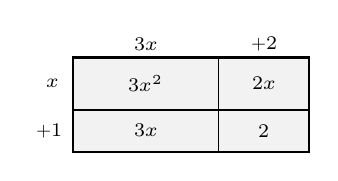
\begin{tikzpicture}[x=1cm, y=1cm, every node/.style={font=\scriptsize, text=black}]
      \draw[black, line width=0.85pt, fill=gray!10] (0.55,0.15) rectangle (3.55,1.35);
      \draw[black, line width=0.6pt] (2.40,0.15) -- (2.40,1.35);
      \draw[black, line width=0.6pt] (0.55,0.68) -- (3.55,0.68);
      \node at (1.48,1.52) {$3x$};
      \node at (2.98,1.52) {$+2$};
      \node at (0.30,1.02) {$x$};
      \node at (0.26,0.42) {$+1$};
      \node at (1.48,1.02) {$3x^2$};
      \node at (2.98,1.02) {$2x$};
      \node at (1.48,0.42) {$3x$};
      \node at (2.98,0.42) {$2$};
    \end{tikzpicture}
  \end{minipage}\hfill
  \begin{minipage}[c]{13.6cm}
    $\bullet$ \textbf{១) គុណឯកធានឹងពហុធា (គំរូទី១ ទំ.៦០)៖}\\[2pt]
    \hspace*{0.25cm}$3x^2(4x^3 + xy - 5y^2) = 3x^2(4x^3) + 3x^2(xy) - 3x^2(5y^2) =$ \ansbox[4.8cm]\\[3pt]
    $\bullet$ \textbf{២) គុណពហុធានឹងពហុធា (ផ្ទៃរូបថតប្រាសាទ ទំ.៥៩)៖}\\[2pt]
    \hspace*{0.25cm}$(3x + 2)(x + 1) = 3x^2 + 3x + 2x + 2 =$ \ansbox[4.2cm]
  \end{minipage}
\end{tcolorbox}

\vspace{4pt}
\textbf{សកម្មភាព ២ (\en{E2-B} — ៦ នាទី)៖ ចែកពហុធានឹងឯកធា និងចែកពហុធានឹងពហុធា (ទំ.៦០--៦១)}

\begin{tcolorbox}[
  enhanced, sharp corners, colback=white, colframe=black,
  boxrule=0.8pt, boxsep=2.5pt, top=4pt, bottom=4pt, left=6pt, right=6pt
]
  $\bullet$ \textbf{១) ចែកពហុធានឹងឯកធា (ទំ.៦០)៖} $(6x^3 + 8x^2 + 10x) \div (2x) = \dfrac{6x^3}{2x} + \dfrac{8x^2}{2x} + \dfrac{10x}{2x} =$ \ansbox[4.2cm]\\[4pt]
  $\bullet$ \textbf{២) ចែកពហុធានឹងពហុធាតាមជួរឈរ (ឧទាហរណ៍ទី ៣ និងទី ៤ ទំ.៦១)៖}\\[2pt]
  \hspace*{0.3cm}-- $(x^2 - 7x + 10) \div (x - 2) =$ \ansbox[2.8cm] (សំណល់ $R =$ \dotline[1.0cm] ហៅថា\textbf{ចែកដាច់})\\[2pt]
  \hspace*{0.3cm}-- $(x^2 - 2x + 4) \div (x - 1) =$ \dotline[2.4cm] $+ \dfrac{\dotline[0.9cm]}{x - 1}$ (ផលចែក $Q = x - 1$, សំណល់ $R =$ \dotline[1.0cm])
\end{tcolorbox}

\vfill

% --- E3 Explain ---
\secstrip{ផ្នែកទី ៣ \enbf{(E3 - Explain)} ៖ ក្បួនគោល និងធនាគារហេតុផល \enbf{B\&W}}{រយៈពេល ៦ នាទី}

\begin{tcolorbox}[
  enhanced, sharp corners, colback=white, colframe=black,
  boxrule=0.85pt, boxsep=2.5pt, top=4pt, bottom=4pt, left=6pt, right=6pt
]
  $\bullet$ \textbf{១) គុណពីរពហុធា៖} គុណតួនីមួយៗនៃពហុធាទី១ នឹងគ្រប់តួនៃពហុធាទី២ រួចបង្រួម \dotline[3.0cm] ។\\[3pt]
  $\bullet$ \textbf{២) ចែកពហុធានឹងឯកធា៖} ចែក\textbf{គ្រប់តួទាំងអស់}នៃពហុធានឹងឯកធានោះ រួច \dotline[3.2cm] ។\\[3pt]
  $\bullet$ \textbf{៣) ចែកពហុធា $A$ នឹង $B$៖} $\dfrac{A}{B} = Q + \dfrac{R}{B}$ ដែលដឺក្រេនៃសំណល់ $R$ តូចជាង \dotline[3.2cm] ។\\[4pt]
  \tikz\draw[black, dashed, line width=0.5pt] (0,0) -- (18.4cm,0);\\[3pt]
  \fontsize{8.8pt}{13.0pt}\selectfont
  \textbf{ធនាគារហេតុផល (\en{Warrant Bank})៖} \quad
  \cnum{1} គុណបំបែកគ្រប់គូតួ ($-\times - = +$) \quad
  \cnum{2} រៀបពហុធាតាមដឺក្រេចុះមុនគុណ/ចែកជួរឈរ\\
  \cnum{3} ចែកគ្រប់តួនឹងឯកធា (តួចែកនឹងខ្លួនឯងស្មើ $\pm 1$) \quad
  \cnum{4} ថែមតួ $0x^k$ ចំពោះខ្ទង់ដែលបាត់ពេលចែកជួរឈរ
\end{tcolorbox}

% ============================================================================
% ទំព័រទី ២៖ សន្លឹកកិច្ចការសិស្ស (ផ្នែកខាងខ្នង៖ E4 -> E5 -> កិច្ចការផ្ទះ)
% ============================================================================
\clearpage
\pagebanner{សន្លឹកកិច្ចការសិស្ស \enbf{(}៥\enbf{.}២\enbf{.}៤\enbf{--}៥\enbf{.}២\enbf{.}៥ វិធីគុណនិងចែកពហុធា\enbf{)} \enbf{--} ផ្នែកខាងខ្នង}{ថ្នាក់ទី៨ \en{|} សៀវភៅគោល ទំ.៦០--៦២, ៧២--៧៣}

% --- E4 Elaborate ---
\secstrip{ផ្នែកទី ៤ \enbf{(E4 - Elaborate)} ៖ លំហាត់គំរូគុណជួរឈរ និងចែកពហុធាបាត់ខ្ទង់ (ទំ.៦០--៦២)}{រយៈពេល ១០ នាទី}

\begin{tcolorbox}[
  enhanced, sharp corners, colback=white, colframe=black,
  boxrule=0.8pt, boxsep=2.5pt, top=4pt, bottom=4pt, left=6pt, right=6pt
]
  \textbf{១) គុណពហុធាតាមជួរឈរ និងពហុធាគោល $10$ (លំហាត់គំរូទី ២--៣ ទំ.៦០)៖}\\[3pt]
  \hspace*{0.3cm}$\bullet$ រៀប $(1 + x^2 - 3x)(2x - 3) = (\dotline[2.6cm])(2x - 3) =$ \ansbox[5.2cm]\\[3pt]
  \hspace*{0.3cm}$\bullet$ សរសេរ $7\,368$ ជាពហុធានៃ $10$៖ $7\,368 = 7\times 10^3 +$ \dotline[1.8cm] $+$ \dotline[1.8cm] $+ 8$\\[5pt]
  \textbf{២) ចែកពហុធាដែលបាត់ខ្ទង់កណ្ដាល (លំហាត់គំរូទី ១--២ ទំ.៦១--៦២)៖}\\[3pt]
  \hspace*{0.3cm}$\bullet$ $(8y^3 + 4y^2 + 0y - 7) \div (2y + 3) =$ \ansbox[3.8cm] $- \dfrac{25}{2y + 3}$\\[3pt]
  \hspace*{0.3cm}$\bullet$ $(x^3 + 0x^2 + 0x - 2) \div (x - 1) =$ \ansbox[3.8cm] $- \dfrac{\dotline[0.9cm]}{x - 1}$\\[3pt]
  \fontsize{8.8pt}{13.0pt}\selectfont
  \textbf{ឆ្លុះបញ្ចាំង (\en{EIA Looking-Back})៖} ពេលចែក $(a^2b^3 + 2ab)\div(ab)$ ហេតុអ្វីចម្លើយស្មើ $ab^2 + 2$ មិនមែនស្មើ $ab^2$? \textbf{ព្រោះ} \dotline[2.8cm] ។\\[4pt]
  {\renewcommand{\arraystretch}{1.35}
  \begin{tabular}{|L{8.85cm}|L{8.85cm}|}
    \hline
    \cellcolor{headgray}\textbf{ប្រអប់គណនាជួរឈរ $(x^2 - 3x + 1)(2x - 3)$} & \cellcolor{headgray}\textbf{ប្រអប់ចែកជួរឈរ $(x^3 + 0x^2 + 0x - 2) \div (x - 1)$} \\ \hline
    ជំហាន ១៖ $(x^2-3x+1)\times(-3) =$ \dotline[3.6cm] & ជំហាន ១៖ $x^3 \div x = x^2 \implies -(x^3 - x^2) \to$ សល់ \dotline[1.6cm] \\
    ជំហាន ២៖ $(x^2-3x+1)\times(2x) =$ \dotline[3.6cm] & ជំហាន ២៖ ទម្លាក់ $+0x, -2$ ចែកបន្ត បានសំណល់ $R =$ \dotline[1.2cm] \\ \hline
  \end{tabular}}
\end{tcolorbox}

\vspace{4pt}

% --- E5 Evaluate ---
\secstrip{ផ្នែកទី ៥ \enbf{(E5 - Evaluate)} ៖ ប្រតិបត្តិ (ទំ.៦០, ៦២) សំណួរវិនិច្ឆ័យ \enbf{A--D} និងសំបុត្រចេញ}{រយៈពេល ១០ នាទី}

\begin{tcolorbox}[
  enhanced, sharp corners, colback=white, colframe=black,
  boxrule=0.8pt, boxsep=2.5pt, top=4pt, bottom=4pt, left=6pt, right=6pt
]
  \textbf{១) ប្រតិបត្តិជាក្រុម (ទំ.៦០ និង ទំ.៦២)៖}\\[3pt]
  \hspace*{0.3cm}$\bullet$ ទំ.៦០ (ក)៖ $2x^2(2x^2 + 3x - 1) =$ \ansbox[4.8cm]\\[3pt]
  \hspace*{0.3cm}$\bullet$ ទំ.៦២ (ក)៖ $(a^2b^3 + 2ab) \div (ab) =$ \ansbox[3.0cm] \qquad
  ទំ.៦២ (គ)៖ $(6x^2 + 5x - 4) \div (2x - 1) =$ \ansbox[3.0cm]\\[4pt]
  \textbf{២) បិទបេសកកម្ម \en{E1}៖} សិស្ស \dotline[1.0cm] ត្រឹមត្រូវ ព្រោះ $(15x^4 - 30x^6)\div(5x^2) =$ \ansbox[3.8cm] ។
\end{tcolorbox}

\vspace{4pt}

\begin{tcolorbox}[
  enhanced, sharp corners, colback=white, colframe=black,
  boxrule=0.8pt, boxsep=2.5pt, top=4pt, bottom=4pt, left=6pt, right=6pt
]
  \textbf{៣) សំណួរវិនិច្ឆ័យ \en{A--D} (គណនា $(12x^3 - 6x) \div (6x)$ — គូសរង្វង់ រួចលើកម្រាមដៃ ១--៤)៖}\\[3pt]
  \textbf{\en{A.}} $2x^2 - 6x$ \qquad\qquad
  \textbf{\en{B.}} $2x^2$ \qquad\qquad
  \textbf{\en{C.}} $2x^2 - 1$ \qquad\qquad
  \textbf{\en{D.}} $6x^2 - 1$\\[4pt]
  \tikz\draw[black, dashed, line width=0.5pt] (0,0) -- (18.4cm,0);\\[3pt]
  \textbf{៤) សំបុត្រចេញ ៦០ វិនាទី៖} ពន្លាតផលគុណ $(x + 2)(x - 5) =$ \ansbox[4.5cm] ។
\end{tcolorbox}

\vfill

% --- Homework ---
\begin{tcolorbox}[
  enhanced, sharp corners, colback=panelgray, colframe=black,
  boxrule=0.95pt, boxsep=2pt, top=3.5pt, bottom=3.5pt, left=6pt, right=6pt
]
  {\muol\fontsize{9.0pt}{13.0pt}\selectfont កិច្ចការផ្ទះ \enbf{(}សៀវភៅគោល ទំ.៦០, ៦២ និង ទំ.៧២--៧៣ លេខ ២, ៦\enbf{)}}\\[2.5pt]
  \fontsize{8.8pt}{13.0pt}\selectfont
  $\bullet$ \textbf{១) ប្រតិបត្តិទំ.៦០ (គ, ង) និង ទំ.៦២ (ខ, ឃ)៖} គណនា $(a^2+2ab)(a-b)$, $\dfrac{1}{2}xy^2\left(\dfrac{2}{3}xy-3\right)$, $(5x^2y^4+2x^3y^5-12x^2y^2)\div(x^2y^2)$ និង $(a^2+6a-55)\div(a-5)$ ។\\
  $\bullet$ \textbf{២) ទំ.៧២ \#2 និង ទំ.៧៣ \#6៖} សរសេរ $1997$ និង $2674$ ជាពហុធាដឺក្រេចុះនៃ $10$; និងបង្រួម $a(x-b)-b(a-x)+x(a+b)$ ។
\end{tcolorbox}

% ============================================================================
% ទំព័រទី ៣៖ ទំព័រគ្រូបង្រៀន (គំរូប្លង់ក្ដារខៀន ៣ ផ្នែក + ចម្លើយផ្ទៀងផ្ទាត់រហ័ស)
% ============================================================================
\clearpage
\pagebanner{ទំព័រគ្រូបង្រៀន ៖ ប្លង់ក្ដារខៀន \enbf{(}គ្មាន \enbf{LCD)} និងចម្លើយផ្ទៀងផ្ទាត់រហ័ស}{៥.២.៤--៥.២.៥ វិធីគុណនិងចែកពហុធា (\en{ALG54})}

\secstrip{១. គំរូប្លង់បែងចែកក្ដារខៀន ៣ ផ្នែក សម្រាប់ថ្នាក់រៀនគ្មាន \enbf{LCD}}{សម្រាប់គ្រូប្រើដីស/ហ្វឺត}

\begin{center}
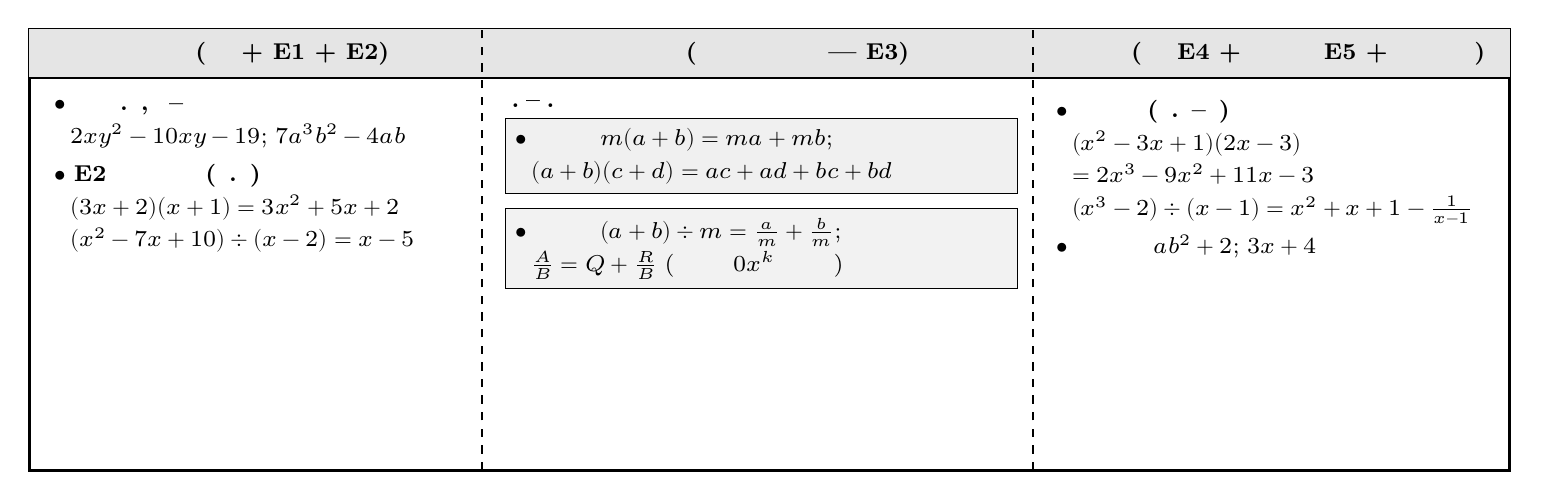
\begin{tikzpicture}[x=1cm, y=1cm, every node/.style={font=\fontsize{8.3pt}{11.8pt}\selectfont, text=black}]
  \draw[black, line width=1.1pt] (0,0) rectangle (18.8,5.60);
  \fill[gray!20] (0,4.98) rectangle (18.8,5.60);
  \draw[black, line width=0.7pt] (0,4.98) -- (18.8,4.98);
  \draw[black, dashed, line width=0.7pt] (5.75,0) -- (5.75,5.60);
  \draw[black, dashed, line width=0.7pt] (12.75,0) -- (12.75,5.60);

  \node at (2.875,5.29) {\textbf{ផ្នែកឆ្វេង (កំណែ + \en{E1} + \en{E2})}};
  \node at (9.25,5.29) {\textbf{ផ្នែកកណ្ដាល (ខ្លឹមសារគោលរក្សាទុក — \en{E3})}};
  \node at (15.775,5.29) {\textbf{ផ្នែកស្ដាំ (គំរូ \en{E4} + ប្រតិបត្តិ \en{E5} + កិច្ចការផ្ទះ)}};

  % Left
  \node[anchor=north west, text width=5.35cm] at (0.20,4.82) {%
    $\bullet$ \textbf{កំណែ ទំ.៥៩, ៧២--៧៣៖}\\
    \hspace*{0.2cm}$2xy^2-10xy-19$; $7a^3b^2-4ab$\\[2pt]
    $\bullet$ \textbf{\en{E2} គំរូផ្ទៃក្រឡា (ទំ.៥៩)៖}\\
    \hspace*{0.2cm}$(3x+2)(x+1) = 3x^2+5x+2$\\
    \hspace*{0.2cm}$(x^2-7x+10)\div(x-2) = x-5$
  };

  % Center
  \node[anchor=north west, text width=6.65cm] at (5.92,4.82) {%
    {\muol\fontsize{8.5pt}{12pt}\selectfont ២\enbf{.}៤\enbf{--}២\enbf{.}៥ គុណនិងចែកពហុធា}\\[3pt]
    \tikz\node[draw=black, fill=gray!12, inner sep=3.5pt, text width=6.25cm]{%
      $\bullet$ \textbf{គុណពហុធា៖} $m(a+b)=ma+mb$;\\
      \hspace*{0.2cm}$(a+b)(c+d) = ac+ad+bc+bd$
    };\\[4pt]
    \tikz\node[draw=black, fill=gray!10, inner sep=3.5pt, text width=6.25cm]{%
      $\bullet$ \textbf{ចែកពហុធា៖} $(a+b)\div m = \tfrac{a}{m}+\tfrac{b}{m}$;\\
      \hspace*{0.2cm}$\tfrac{A}{B} = Q + \tfrac{R}{B}$ (ថែមខ្ទង់ $0x^k$ បើបាត់តួ)
    };
  };

  % Right
  \node[anchor=north west, text width=5.8cm] at (12.92,4.82) {%
    $\bullet$ \textbf{លំហាត់គំរូ (ទំ.៦០--៦២)៖}\\
    \hspace*{0.2cm}$(x^2-3x+1)(2x-3)$\\
    \hspace*{0.2cm}$= 2x^3-9x^2+11x-3$\\
    \hspace*{0.2cm}$(x^3-2)\div(x-1) = x^2+x+1-\tfrac{1}{x-1}$\\[2pt]
    $\bullet$ \textbf{ប្រតិបត្តិ៖} $ab^2+2$; $3x+4$
  };
\end{tikzpicture}
\end{center}

\vspace{4pt}
\secstrip{២. ចម្លើយផ្ទៀងផ្ទាត់រហ័សសម្រាប់សន្លឹកកិច្ចការសិស្ស \enbf{(}ទំព័រ ១ និង ទំព័រ ២\enbf{)}}{\en{Answer Key}}

\begin{tcolorbox}[
  enhanced, sharp corners, colback=white, colframe=black,
  boxrule=0.8pt, boxsep=2pt, top=4pt, bottom=4pt, left=6pt, right=6pt
]
  \fontsize{9.0pt}{13.5pt}\selectfont
  $\bullet$ \textbf{ផ្នែក \en{E1}៖} \textbf{សិស្ស ខ} ត្រឹមត្រូវ ($3x^2 - 6x^4$) ព្រោះត្រូវចែកគ្រប់តួទាំងពីរនៃពហុធានឹង $5x^2$ ។\\[2pt]
  $\bullet$ \textbf{ផ្នែក \en{E2}៖} \textbf{សកម្មភាព ១៖} $12x^5 + 3x^3y - 15x^2y^2$; $3x^2 + 5x + 2$ ។ \textbf{សកម្មភាព ២៖} $3x^2+4x+5$; $x-5$ ($R=0$); $x-1+\frac{3}{x-1}$ ($R=3$) ។\\[2pt]
  $\bullet$ \textbf{ផ្នែក \en{E4}៖} ១) $(x^2-3x+1)(2x-3) = 2x^3-9x^2+11x-3$; $3\times 10^2 + 6\times 10$; ២) $4y^2-4y+6$; $x^2+x+1-\frac{1}{x-1}$ ។\\[2pt]
  $\bullet$ \textbf{ផ្នែក \en{E5}៖} ១) $4x^4+6x^3-2x^2$; $ab^2+2$; $3x+4$; ២) សិស្ស ខ ($3x^2-6x^4$); ៣) \textbf{ជម្រើស \en{C}} ($2x^2-1$); ៤) $x^2 - 3x - 10$ ។
\end{tcolorbox}

\vspace{4pt}
\secstrip{៣. ចម្លើយលម្អិតនៃកិច្ចការផ្ទះ \enbf{(}សម្រាប់ផ្ទៀងនៅដើមម៉ោងបន្ទាប់ ៥\enbf{.}៣\enbf{.}១\enbf{)}}{សៀវភៅគោល ទំ.៦០, ៦២, ៧២--៧៣}

\begin{tcolorbox}[
  enhanced, sharp corners, colback=white, colframe=black,
  boxrule=0.8pt, boxsep=2pt, top=4pt, bottom=4pt, left=6pt, right=6pt
]
  \fontsize{8.8pt}{13.2pt}\selectfont
  $\bullet$ \textbf{១) ទំ.៦០ (គ)៖} $(a^2+2ab)(a-b) = \mathbf{a^3 + a^2b - 2ab^2}$; \quad \textbf{(ង)៖} $\mathbf{\tfrac{1}{3}x^2y^3 - \tfrac{3}{2}xy^2}$; \quad \textbf{ទំ.៦២ (ខ)៖} $\mathbf{5y^2 + 2xy^3 - 12}$; \quad \textbf{(ឃ)៖} $\mathbf{a + 11}$ ។\\[2pt]
  $\bullet$ \textbf{២) ទំ.៧២ \#2៖} $1997 = 1\times 10^3+9\times 10^2+9\times 10+7$, \ $2674 = 2\times 10^3+6\times 10^2+7\times 10+4$; \quad \textbf{ទំ.៧៣ \#6៖} $ax-ab-ab+bx+ax+bx = \mathbf{2ax + 2bx - 2ab}$ ។
\end{tcolorbox}

\end{document}
